\documentclass[a4paper,11pt]{article}

\usepackage[T1]{fontenc}
\usepackage[active]{srcltx}
\usepackage[english]{babel}
\usepackage[numbers]{natbib}
\usepackage[utf8]{inputenc}
\usepackage{amsmath}
\usepackage{amssymb}
%\usepackage{fullpage}
\usepackage{graphicx}
\usepackage{listings}
\usepackage{parskip}
\usepackage{srcltx}
\usepackage{url}

\urlstyle{same}

\newcommand{\m}[1]{\boldsymbol{#1}}
\renewcommand{\*}[0]{\cdot}
\renewcommand{\Pr}[1]{\mathbf{Pr}[#1]}
\renewcommand{\v}[1]{\vec{#1}}
\newcommand{\trans}[2][eng.]{(#1 \emph{#2})}

\title{
    {\sc DD2380 Artificial intelligence} \\
    Project report from group PIMP
}
\author{
    Joel Bohman \\ 881117 \and
    Samuel Lidén Borell \\ 881230 \and
    Joel Pettersson \\ 880519 \and
    Linus Wallgren \\ 880213
}
\date{\today}

\begin{document}
\maketitle
\thispagestyle{empty}
\newpage
\begin{abstract}
    % TODO write abstract
\end{abstract}
\thispagestyle{empty}
%\mbox{}
%\thispagestyle{empty}
\newpage
\setcounter{page}{1}


\part*{Introduction and background}

% - Some kind of introduction and one or two paragraphs about current solvers.
% - Short introduction to the problem and a description of the relationship to
%   the course material. also present what you think are your biggest
%   contributions so that this is clear. be sure to credit anyone that you got
%   help/code from

Sokoban is a puzzle created in 1981 by Hiroyuki Imabayashi. Sokoban is a
difficult puzzle and it has been proven that it is
PSPACE-complete~\cite{culberson1997}, which is a superset of NP. Current
solvers use techniques such as Iterative Deepening Search (IDS), Depth First
Search (DFS), Breadth-First Search (BFS), A* and combination of them to
traverse the search tree. Sokoban has a large branching factor which result in
a large search tree. To be able to traverse the search tree in any reasonable
time, pruning techniques and heuristics are necessary.  Humans can solve
Sokoban puzzles by advanced heuristics that becomes natural to us after playing
the game for a while.  


\section{Problem statement}

% a clear formalization of the problem using course material: which methods, how and why

Our task is to implement a program that is able to solve as many Sokoban levels
as possible. We have received test data that contains 136 levels to test our
solver against. However, we are not supposed to specialize our solver(s) for
this set of levels.


\part*{Theory and method}

\section{Solvers}

\subsection{IDSPusher}

\subsection{IDSPuller}

\subsection{Bidirectional search using IDSPusher and IDSPuller}

\section{Pruning techniques}

\subsection{Repeated states}

\subsubsection{Zobrist keys}

\subsection{Deadlock}

\subsubsection{Dead squares deadlock}

\subsubsection{Freeze deadlock}

\subsection{No influence pushes --- tunnels}

\section{Heuristics}

\subsection{Lower bound}

\subsection{Choosing solver}


\part*{Results}


\part*{Discussion}

\section{Further improvements}

\subsection{A* and search heuristics}

\subsection{Corrals}

\subsection{Incremental reachable square search}

\part*{Conclusion}





Test \cite{culberson1997}.

Testing \cite{russell2009}.

Testing \cite{takes2007}.

\begin{figure}[h]
    \begin{center}
        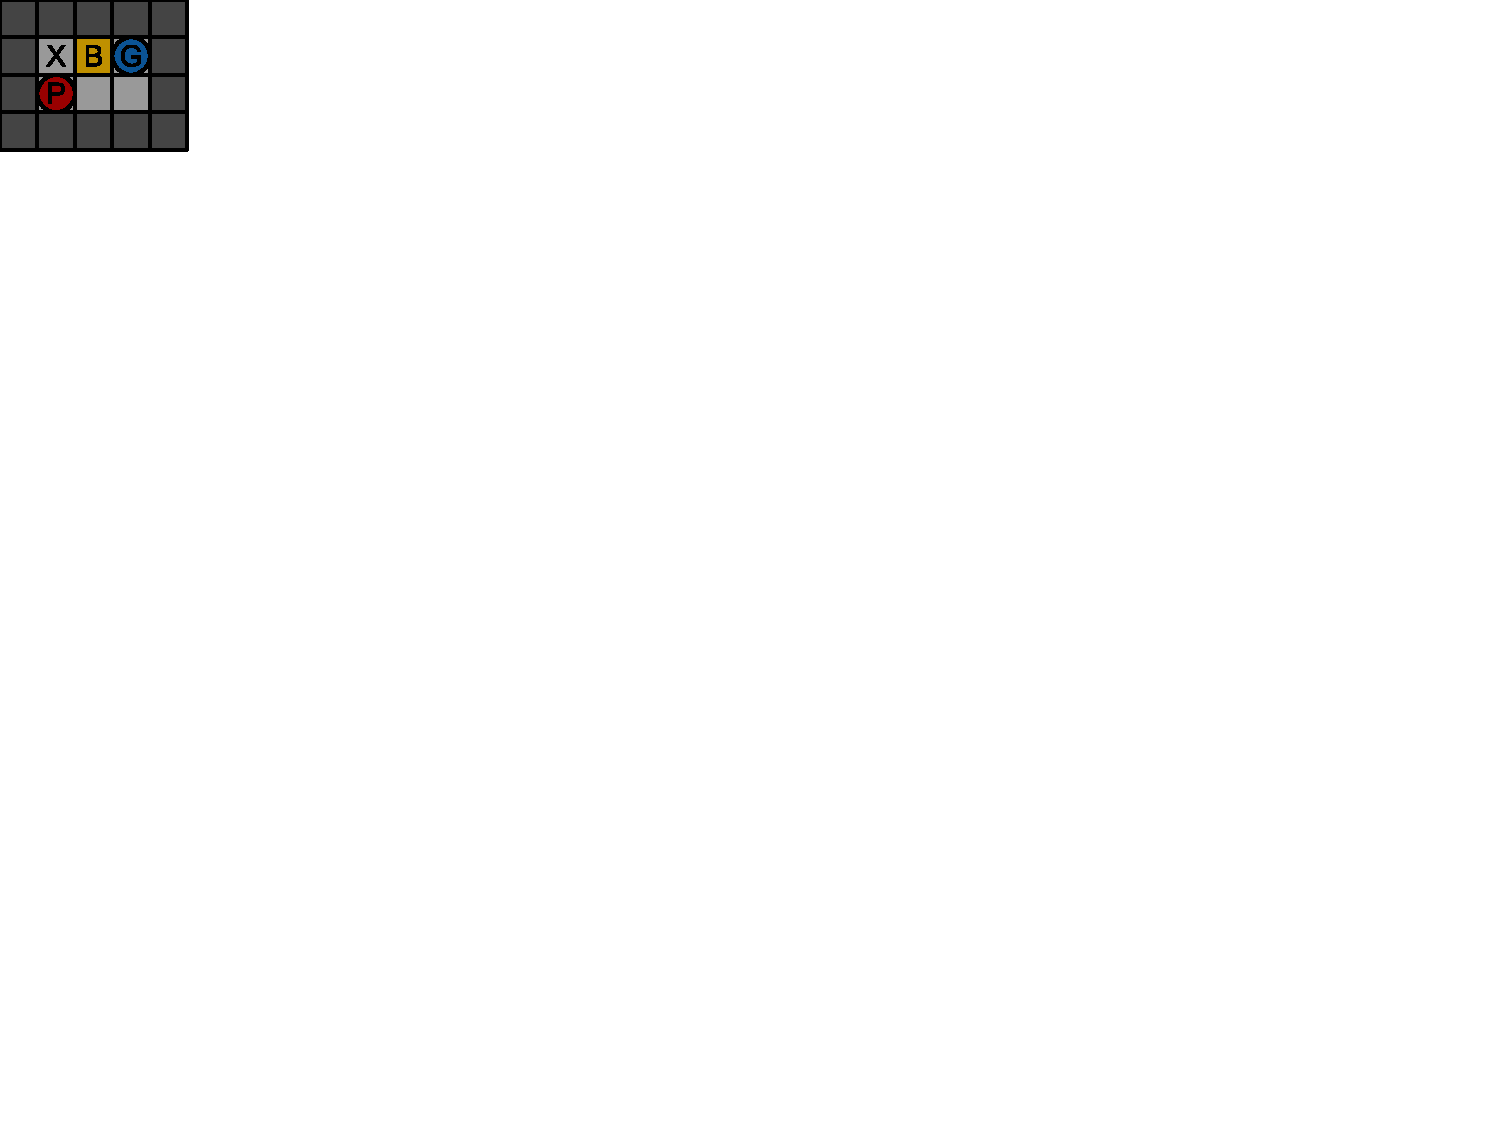
\includegraphics{figures/equalState1}
        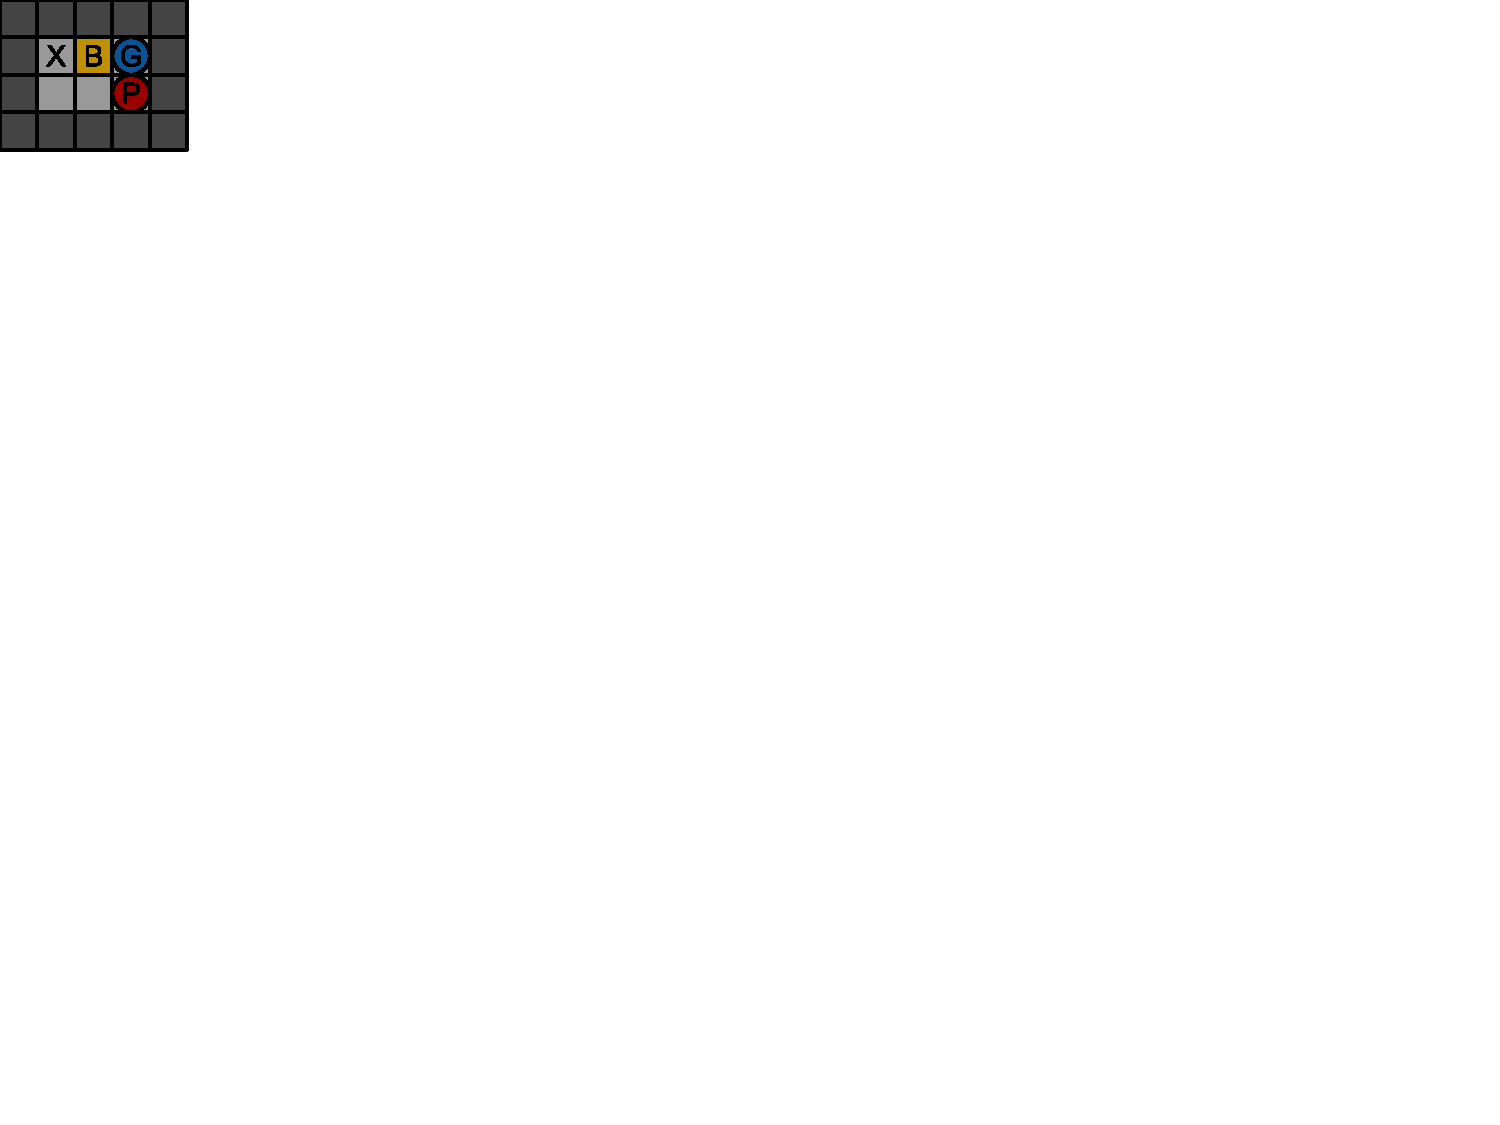
\includegraphics{figures/equalState2}
    \end{center}
    \caption{Test}
    \label{fig:test}
\end{figure}


\bibliographystyle{plainnat}
\bibliography{references} 


\end{document}
